\section{Festplatten- und Flash-Laufwerke}

\subsection{Was sind Festplatten- (HDD) und Flash-Laufwerke (SSD)?}
Beschreiben Sie kurz den Aufbau von und den Zugriff auf HDDs und SSDs.

\begin{solution}
	\begin{minipage}{0.5\linewidth}
		Aufbau HDD:\\
		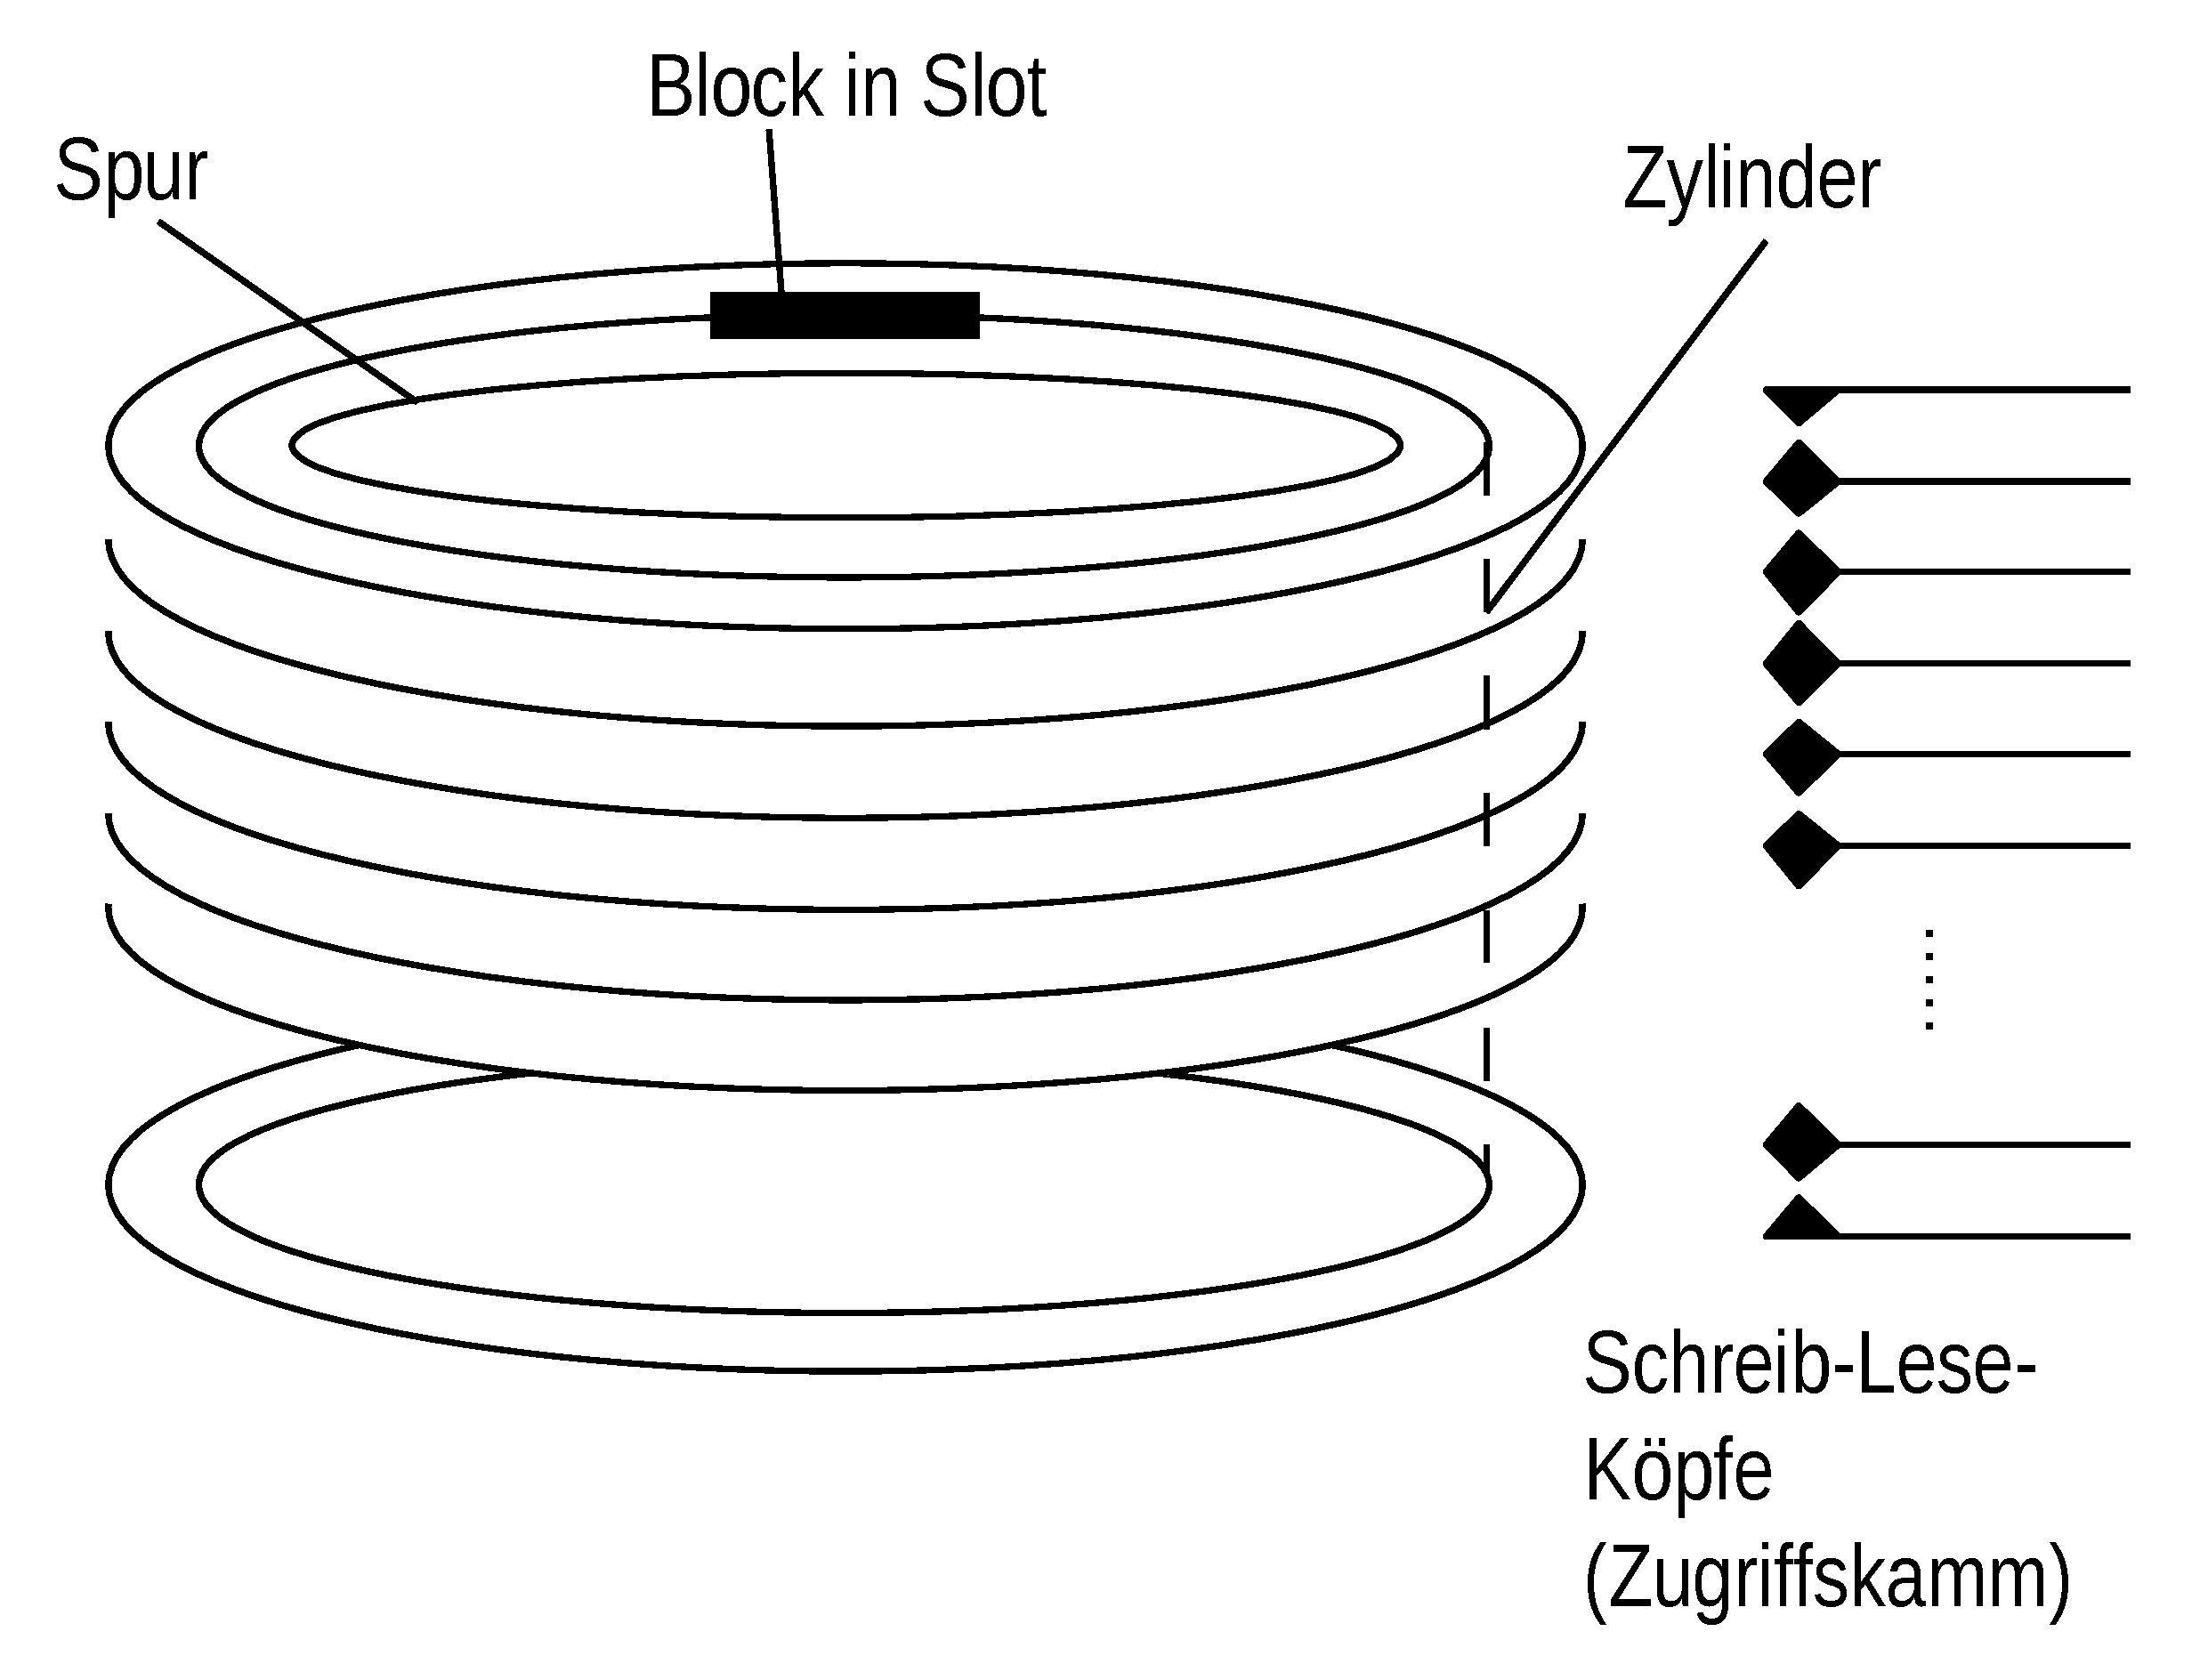
\includegraphics[width=\linewidth]{Pictures/hdd}
	\end{minipage}
	\begin{minipage}{0.49\linewidth}
		Bei einer HDD werden die Blöcke per CHS (\textit{Cylinder}, \textit{Head} (Lesekopf, alternativ \textit{Track} (Spur)), und \textit{Sector} (Slot)) adressiert.
		Der Zugriff auf den ersten Block hat einen hohen Aufwand, da der Lesekopf zunächst auf die richtige Spur ausgerichtet werden muss (Seek-Zeit).
		Anschließend muss (kurz) darauf gewartet werden, bis sich die Platte bis zum richtigen Slot gedreht hat.
		Folgeblöcke aus der selben Spur können dafür aber relativ schnell ausgelesen werden.
		Der Wechsel zu einem anderen Lesekopf/ einer Nachbarspur erfordert ein kurzes Neueinstellen des Zugriffskamms (Track-to-Track-Zeit).
	\end{minipage}
	Bei einer SSD sind die Slots in Speicherchips und Blöcke aufgeteilt.
	Mithilfe mehrerer Speicherchips kann parallel auf das Laufwerk zugegriffen werden.
	Die Blöcke bezeichnen die \textit{kleinste löschbare Einheit}, diese umfasst mehrere Slots und ist meist mehrere Megabyte groß.
	Da das Löschen nur auf dem gesamten Block geschieht wird die  Blockadresse nicht linear auf Slots abgebildet.
	Das Auslesen eines Slots geschieht ohne physische Bewegung, sondern direkt (Leselatenz).
	Sequentielle Zugriffe können zu einem gebündelt werden, wodurch diese beschleunigt werden.
	Weitere Infos zu SSDs können Sie in diesem Blogbeitrag nachlesen: \href{http://databasearchitects.blogspot.com/2021/06/what-every-programmer-should-know-about.html}{databasearchitects.blogspot.com/2021/06/what-every-programmer-should-know-about.html}
\end{solution}

\beamertxt{\pagebreak}
\subsection{Zugriffszeiten}
\label{ZugriffFestplatten}
Stellen Sie sich vor, Sie haben Laufwerke mit folgenden Leistungsdaten:

\begin{minipage}[t]{0.55\linewidth}
	\paragraph{HDD Seagate~Ironwolf~Pro 18~TB (ST18000NE0000)}
	\begin{itemize}
		\item 480.000 Zylinder
		\item 18 Spuren pro Zylinder
		\item 4064 Sektoren pro Spur
		\item 512 Byte pro Sektor
		\item 7200 RPM
		\item Durchschnittliche Latenz: 4.16 ms
		\begin{itemize}
			\item Track-to-Track-Zeit (Annahme): 0,2ms
		\end{itemize}
		\item Kosten 367€ (06/2023)

	\end{itemize}
\end{minipage}
\hfill
\begin{minipage}[t]{0.35\linewidth}
	\paragraph{SSD Seagate FireCuda 530 4TB (ZP4000GM30013)}
	\begin{itemize}
		\item Random Read (Parallel): 1.000.000 IOPS\normaltxt{ (Input / Output Operations Per Second)}, 4KiB Einheiten
		\begin{itemize}
			\item Leselatenz (Annahme): 80µs
		\end{itemize}
		\item Sequential Read: 7300~MB/s, 128~KiB Einheiten
		\item Kosten 377€ (06/2023)
	\end{itemize}
\end{minipage}



\paragraph{Aufgabe}
\begin{enumerate}[a)]
	\item Wie lange benötigen Sie im Mittel, um 10.000 Blöcke (4 KiB, also ca. 39MiB)
	\label{ZugriffFestplattenDauern}

	\begin{enumerate}[i)]
		\item sequentiell zu lesen?

		\begin{solution}
			\begin{description}
				\item[Festplattenlaufwerk]
				\begin{note}
					Evtl vorher berechnen:
					\begin{itemize}
						\item Zeit pro Umdrehung (60s/7200) = 8,33ms
						\item Blöcke pro Spur = 4064/8 = 508
					\end{itemize}
				\end{note}
				Für den Zugriff auf einen beliebigen Slot benötigt es die durchschnittliche Latenz ($T_{Zugriff}$ = 4.16~ms)

				Im Anschluss kann die ganze Spur in $T_{Rotation}$ gelesen werden.
				Doch wie viele Spuren müssen gelesen werden?
				\begin{align*}
					\textit{Blöcke pro Spur} &= \textit{Sektoren pro Spur} / \textit{Sektoren pro Block} = 4064/8 = 508\\ 
					\textit{Anzahl an Spuren} &= \textit{Anzahl an Blöcken} / \textit{Blöcke pro Spur}\\
					&= 10.000 / 508 \approx 19,69
				\end{align*}
				Damit müssen 18 bis 19 volle Spuren und bis zu zwei Spuren anteilig gelesen werden.
				Im einfachsten Fall haben wir eine erste volle Spur, weitere 18 volle Spuren und eine zusätzliche Spur für den Rest.
				Um zwischen 2 benachbarten Spuren zu wechseln fällt keine ganze $T_{Zugriff}$ an, sondern lediglich eine $T_{Track2Track}$.
				Die unvollständige Spur hat in Größe von $10.000 - 19*508 = 348$ Blöcke.
				Damit erhalten wir:
				\begin{align*}
					T_{10.000} &= T_{erste Spur} + 18\cdot T_{ganze Zusätzliche Spur Lesen} + T_{letzte Spur}\\
					&= T_{Zugriff} + T_{Rotation}\\
					&+ 18 (T_{Track2Track}  + T_{Rotation})\\
					&+ T_{Track2Track} + T_{Lesen Letzte Spur}\\
					&= T_{Zugriff} + T_{Lesen Letzte Spur}\\
					&+ 19 (T_{Track2Track}  + T_{Rotation})\\
					&= 4,16ms + 348/508 \cdot 8,33 ms\\
					&+ 19 \cdot (0,2ms + 8,33ms)\\
					&\approx 9,87 + 162,07ms  \approx 172ms
				\end{align*}
				\item[Flashlaufwerk]
				Für 10.000 Blöcke der Größe 4KiB benötigen wir $10.000/(128/4) = 312,5$ also 313 bis 314 Einheiten.
				Wie lange dauert es, eine Einheit zu lesen?
				\begin{align*}
					T_{SequenzielleEinheit} &= 128KiB/7300 MB/s\\
					&= (128 \cdot 1024) /(7300 \cdot 1000\cdot 1000) s  \\
					&\approx 18 \mu s
				\end{align*}
				Damit erhalten wir im schlechtesten Fall $18\mu s \cdot 314 = 5,6ms$
			\end{description}
		\end{solution}


		\item verstreute zu lesen?
		Gehen Sie davon aus, dass die Blöcke völlig zufällig verteilt sind.

		\begin{solution}
			\begin{description}
				\item[Festplattenlaufwerk] 
				Wir gehen in der Musterlösung vom Worst Case aus (= jeder der 10.000 gesuchten Blöcke liegt auf einer anderen zufälligen Spur, was bei 480.000 Spuren nicht unwahrscheinlich ist), d.h. für jeden Block muss $TZugriff$ aufgewendet werden.
				Die Lesezeit für einen Block pro Spur beträgt $1/508$ einer Umdrehung, das ist vernachlässigbar klein.
				Dauer insgesamt: 
				\begin{align*}
					T &= 10000 \cdot ( TZugriff + vernachlaessigbare Lesezeit)\\
					&= 10000 \cdot 4,16ms = 41,6s
				\end{align*}
				\item[Flashlaufwerk]
				Da über jeden NAND-Channel unabhängig zugegriffen werden kann, muss hier der parallele Zugriff vom sequentiellen unterscheiden werden.
				\begin{description}
					\item[sequentiel] Wenn die Blöcke nur einer nach dem anderen zugegriffen werden können, benötigt jeder Block die Leselatenz.
					Damit $10.000\cdot 80\mu s = 800 ms$
					\item[parallel] Beim lesen von 10.000 Blöcken benötigt die SSD jeweils eine IOP.
					Damit $10.000/1.000.000 s = 1/100 s = 10 ms$
				\end{description}
			\end{description}
		\end{solution}

		\begin{note}
			Vielleicht kommt jemand auf die Idee, dass ja rein zufällig zwei Blöcke auf dem gleichen Zylinder liegen.
			Das Geburtstagsparadoxon legt das Nahe.
			Bei insgesamt 10000 Blöcken auf über 480.000 Zylindern (*18 Spuren) liegt die wslkt zwar bei $99,7\% $, jedoch machen bei 10000 Zugriffen eine Hand voll eingesparte Zugriffe auch keinen allzu großen Unterschied.
		\end{note}

	\end{enumerate}




	\item Wie bereits erwähnt, sind SSDs und HDDs unterschiedlich aufgebaut.
	Wie könnte eine einheitliche Schnittstelle aussehen, mit der man Blöcke sowohl von Festplatten als auch von SSDs lesen kann?

	\begin{solution}
		Als gemeinsame Schnittstelle kann man auf jedes Gerät über die Blocknummer zugreifen.
		Das implementieren mit LBA (Logical Block Adressing) auch eigentlich alle Speichermedien seit mindestens 1996 (Win98 ist zwar noch auf 128\,GB beschränkt, aber schon mit LBA).

		Das ist schon eine Abstraktion: Wir müssen nicht mehr das physische Layout der Daten auf einem Laufwerk kennen; wenn wir die Größe eines Gerätes kennen, können wir alle Blöcke adressieren.
		Diese Abstraktion ist notwendig, da neuere Laufwerke (z.B. SSD) einen grundlegend anderen Aufbau als ältere Laufwerke (z.B. HDD) haben.
		Auch HDDs sind unter sich unterschiedlich aufgebaut.
		So kann sich die Anzahl der Zylinder, Spuren pro Zylinder, oder Slots pro Spur beim Austausch einer HDD ändern.
		Gleiches gilt übrigens auch für CDs (constant linear velocity vs. constant angular velocity).
	\end{solution}

	\item Was sind die Vorteile beziehungsweise Nachteile von sehr kleinen und sehr großen Blockgrößen innerhalb eines Dateisystems?

	\begin{solution}
		\paragraph{I/O-Operationen}
		Kleine Blockgrößen haben den Nachteil, dass sehr viele I/O-Operationen notwendig (teuer) sind, was bei großen Blockgrößen deutlich weniger wird.
		Außerdem ist der Verwaltungsaufwand bei kleinen Blöcken größer.
		Dafür ist die Platzverschwendung pro Block nicht so groß.

		\paragraph{Speicherplatz}
		Große Blöcke können Speicherplatzverschwendung sein, da man immer einen ganzen Block allokieren muss.
		Wenn z.B. eine Relation sehr klein ist, nutzt sie nicht den ganzen Block aus.
		Umgekehrt bleibt je Block aber im Mittel der Platz für einen halben Satz ungenutzt.
		Somit verschwenden wir bei kleinen Blöcken weniger Platz.
		Das sehen wir aber erst in der nächsten Übung.
	\end{solution}
	\item Bestimmen Sie die Kosten für die genannten Datenspeicher in $\geneuro/GB$.

	\begin{solution}
		\begin{description}
			\item[HDD] $367\geneuro / 18TB = 367 / (1000*18) \cdot \geneuro/GB \approx 0,02 \geneuro/GB$
			\item[SSD] $377\geneuro / 4TB = 377 /(1000*4) \cdot \geneuro/GB \approx 0,09 \geneuro/GB$
		\end{description}
		Wie Sie erkennen können ist SSD-Speicher um weniger als eine Größeneinheit teurer als HDD-Speicher.
	\end{solution}
\end{enumerate}
